\section{Présentation du programme API et mon rôle dans celui-ci}
\label{p2}

    \subsection{Qu'est ce qu'une API ?}

    Le terme API\,\footnote{API : \foreignlanguage{english}{Application Programming Interface}, interface de programmation applicative en français.} est un terme générique identifiant une interface entre deux systèmes, notamment pour des interfaces temps réel web telles que les web-services.
    Attention toutefois, la démarche API et la démarche web-services sont différentes !

    Dans notre cas, une API est techniquement un web-service simple  accessible en self-service (au moins pour sa découverte) ;
    c’est-à-dire que des règles de design précises ont été respectées lors de sa conception (par ex. API REST\,\footnote{REST : \foreignlanguage{english}{Representational state transfer} , un style d'architecture basé sur le protocole HTTP.}\,\up{\cite{octodesign}}).
    Sa documentation est réalisée d’une façon particulière avec beaucoup de soin et un ensemble de bouchons sont disponibles pour réaliser des tests (l'équivalent d'un environnement bac à sable).

    \begin{figure}[!ht]
        \center
        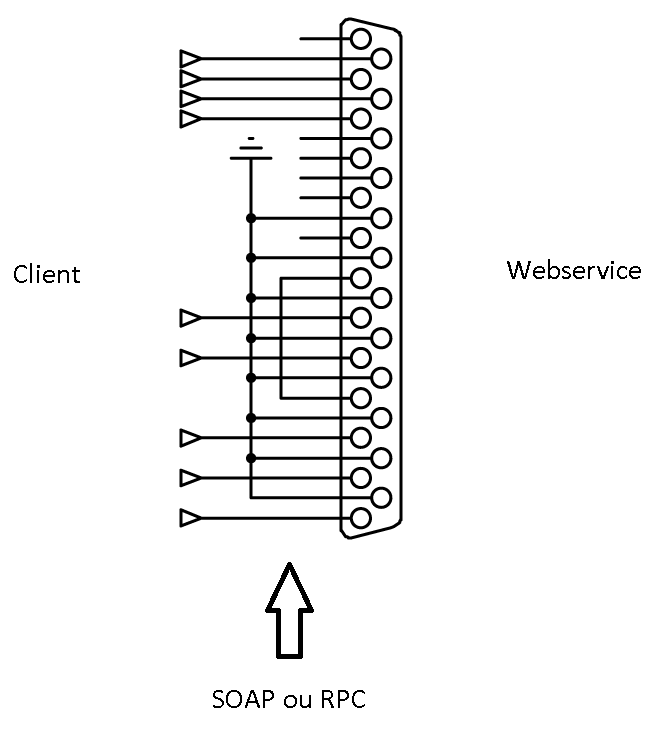
\includegraphics[width=0.5\textwidth]{./images/webservice.jpg}
        \caption{Un webservice typique offre de nombreux points d'entrée complexes}
    \end{figure}

    Le but de la démarche API est d’aller plus loin dans le découplage des applications et des organisations (projet notamment).
    Une API, c’est aussi un langage commun et transverse entre le métier et le SI.
    Résultat : une meilleure agilité, une simplicité et de meilleures performances pour le SI !

    Une API se construit grâce à une démarche commune de partage et de co-construction de tous les acteurs (fonctionnels comme techniques) en mettant dès le départ l'accent sur le design et la documentation.
    Une API est toujours construite dans l’optique qu’elle puisse être rendue publique, sa conception et son accessibilité doivent donc être le plus soignées possible.
    Contrairement aux web-services dotés d’un contrat d’interface complexe et différent pour chaque besoin client, les messages d’une API sont son interface qui lui est  unique, commune et globale.

    \begin{figure}[!ht]
        \center
        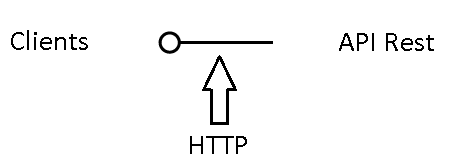
\includegraphics[width=0.35\textwidth]{./images/api-rest.jpg}
        \caption{Une API REST offre un point d'entrée unique et simple}
    \end{figure}

    Une API REST (representational state transfer) est une API client-serveur conçue grâce à une modélisation orientée ressources (et non plus méthodes comme c’était le cas en web-services) avec la contrainte d’être serveur sans état, c’est à dire que chaque message contient toutes les données et informations nécessaires à son traitement, il n’y a pas de contexte créé du coté serveur suite aux enchaînements de requêtes.
    Elle se base aussi sur un protocole de haut niveau omniprésent : HTTP, qui fournit des verbes (méthodes GET POST DELETE PUT ...) ainsi que le système de schéma (URL, URI), cela lui procure une facilité d’usage universelle.
    Nous parlerons maintenant d’API en tant qu’abréviation d’API REST.

    La question que les architectes et designers doivent se poser n’est pas
    “Comment un serveur doit-il exporter ses objets privés de sorte que les clients puissent les comprendre et les utiliser ? “, mais plutôt
    “Comment un client et un serveur peuvent partager une compréhension commune des données brutes échangées entre eux ?”\,\up{\cite{apihtml5}}

    Un client est donc autonome grâce à la simplicité et au self-service (catalogue d’API) ainsi que la robustesse des API induite par leur fort découplage.
    La documentation complète répond à la majorité de ces questions, il peut aussi contacter l’équipe projet pour exprimer ses demandes (demandes qui seront donc évaluées et peut-être ajoutées dans la documentation).

    Le fournisseur d’API l’expose sur une « Gateway », point d’accès et d’exposition central, et y délègue tout ou partie de la gestion des quotas clients.
    Il n’a donc pas à configurer pour chaque client l’interconnexion, le processus est automatisé au maximum possible (en gardant les spécificités métiers s’il y en a).
    Son planning n’est plus dépendant de la synchronisation à chaque souscription d’un client.

    Les API rentrent dans une évolution plus globale des SI, avec de nouvelles architectures, technologies et façon de concevoir les applications.
    C’est la suite logique du SOA (service oriented architecture) dans les systèmes d'informations.
    Ce n’est cependant pas un but mais une démarche !

    \subsection{Le programme API et ses objectifs}

    Le programme API est une équipe constituée de trois personnes :  Yan Delcroix directeur du programme, Yannick Cosson responsable des formations API et moi-même.

    \begin{figure}[!ht]
        \center
        
\includegraphics[width=0.6\textwidth]{./images/api-si-france.jpg}
        \caption{La bannière du programme API}
    \end{figure}

    Les ambitions à sa création était de rendre accessible les principales fonctionnalités et données du SI sous forme d’API simples en mode self-service pour les équipes projets construisant le SI France, ainsi que la valorisation du patrimoine SI en exposant des API publiques pour les développeurs externes permettant de stimuler un écosystème innovant autour du patrimoine d’Orange France.

    Ce programme a pour mission l’accompagnement des projets dans la consommation ou la création d’API, ainsi que la garantie de la mise à dispositions de moyens nécessaire à ces projets, l’animation de la communauté de compétences API et le recueil d’expertise sur le thème des API, la communication autour de ce thème et sa promotion pour augmenter la réutilisation, et le pilotage de la roadmap transverse de déploiement et publication des API.

    Le programme API est aussi constitué d’une communauté composée de référents dans chaque domaine métier et de champions API, ce sont les points de contacts directs et privilégiés dans leur domaine à propos des API.

    Les missions du référent API sont nombreuses. Il porte les besoins et les avancées de son domaine pour faire évoluer opérationnellement la stratégie API, ainsi que la communauté de compétences (par capitalisation globale).
    Il accompagne les équipes projets pour les aider à produire des nouvelles API simples, robustes et accessibles en self-service.
    Il anime aussi les collèges API de co-construction avec les métiers sponsors pour piloter, prioriser et anticiper efficacement les API qui ont le plus de valeur, voir même de définition d’API communes inter-domaine métier, et aussi stimuler et suivre la réutilisation.

    Les champions API, quant à eux, sont des contributeurs projets confirmés dans la conception et la démarche autour des API.

    La validation par la communauté des designs d’API avant leur développement permet de s’assurer de la bonne conception et du respect de contraintes liées aux différentes livrables.

    \subsection{Le rôle d'architecte logiciel}

    Les compétences d’un architecte logiciel sont à la fois des compétences techniques et de la pédagogie.
    Il possède une grande expérience et une vue d’ensemble sur les techniques et technologies mais n’est pas un expert.

    En effet, les architectes logiciels ne peuvent pas être des spécialistes de tous les langages / bibliothèques, par conséquent ils se basent sur des recommandations d’experts.
    Ces dernières sont nombreuses, variées et souvent très complexes.
    L’architecte doit être capable de savoir où chercher et seule son expérience peut l’aider dans cette tâche de veille.

    Toutes les informations utiles au projet ne sont pas standardisées, il doit donc avoir un réseau d’experts auquel s’adresser.
    Chez Orange, les architectes tissent des liens pour établir leur réseau d’experts.
    Cette capacité ne dépend pas d’un processus, mais des qualités propres aux architectes : être sociables et ouverts d’esprits.
    L’architecte écoute, réfléchit, communique, il comprend les besoins du projet et les impacts sur le SI, ce qui lui permet de contacter les personnes compétentes ou responsables et d’échanger avec ces dernières pour tirer des conclusions sur lesquelles il capitalise l’expérience.

    Pour se mettre régulièrement à jour sur les nouvelles préconisations du groupe ou sur une nouveauté technique, les salariés choisissent sur une plateforme les formations ou les présentations auxquelles ils souhaitent participer.
    Ces interventions peuvent être physiques dans des salles ou des amphithéâtres, ou dématérialisées grâce à l’intranet.
    Elles peuvent durer moins d’une heure ou s’étaler sur plusieurs jours.
    Elles ont lieu dans les locaux des salariés ou dans une autre succursale du groupe.
    Ainsi le salarié prend l’initiative de se former.
    Quand les formations durent moins d’une heure, ils n’hésitent pas à les suivre pendant la pause du déjeuner.
    Les architectes qui m’entourent estiment en moyenne que 80 \% de leur temps de travail est dédié au projet et 20 \% à la veille.

    Par son travail de conseil, il doit être capable de transmettre son expertise et son expérience avec un langage compréhensible par les personnes de l’entreprise, se montrer pédagogue, diplomate et patient.

    Travaillant au milieu d’une multitude d’architectes (techniques, fonctionnels, logiciels) je me suis rendu compte que lors des réunions, ces architectes utilisent un ton calme et lent, font attention à la formulation pour ne pas heurter ou perdre leurs interlocuteurs qui ne sont pas toujours initié à la thématique abordée.
